The \textit{Account} module is responsible for management of users using the system. The scope for the \textit{Account} module is shown in Figure 2.  \\[1cm]

\begin{figure}[h]
	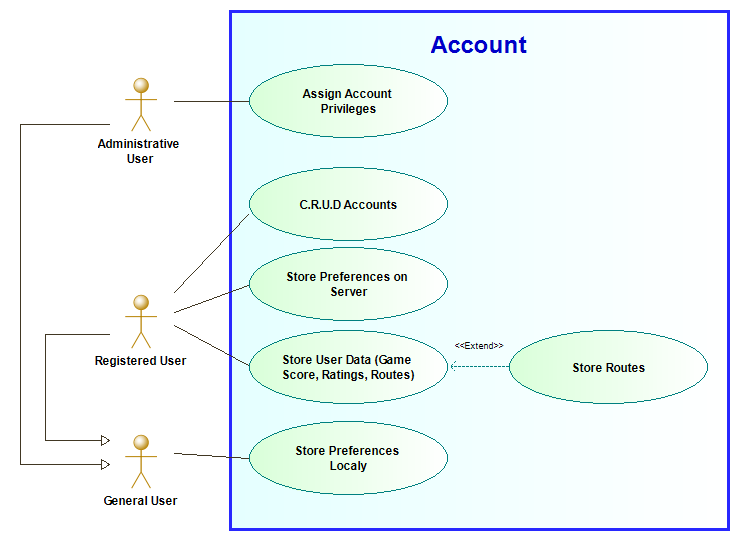
\includegraphics[width=\textwidth]{Account_Use_Case_Diagram}
	\caption{Account module use case}
\end{figure}

\begin{enumerate}
	\item \textbf{Assign Account Privileges}
	\begin{itemize}
		\item Description: \\
		This use case allows the admin user to assign privileges to registered users. He/She may promote or demote users to higher privileges 
		\item Pre-Conditions: \\
		\begin{itemize}
		\item User must be logged in
		\item User must have admin privileges
		\item The admin user must supply a registered user in the request
		
		\end{itemize}
		\item Post-Conditions: \\
		
		\begin{itemize}
		\item The supplied user will have new access privileges 
		
		\end{itemize}
	
	\end{itemize}
	
	\item \textbf{C.R.U.D. Accounts}
	\begin{itemize}
		\item Description: \\
		This use case allow a user to create, update and deactivate an account for the NavUP system
		\item Pre-Conditions: \\
		
		\item Post-Conditions: \\
	
	\end{itemize}
	
	\item \textbf{Store Preferences on Server}
	\begin{itemize}
		\item Description: \\
		
		\item Pre-Conditions: \\
		
		\item Post-Conditions: \\
	
	\end{itemize}
	
	\item \textbf{Store User Data}
	\begin{itemize}
		\item Description: \\
		
		\item Pre-Conditions: \\
		
		\item Post-Conditions: \\
	
	\end{itemize}
	
	\item \textbf{Store Preferences Locally}
	\begin{itemize}
		\item Description: \\
	
		\item Pre-Conditions: \\
		
		\item Post-Conditions: \\
	
	\end{itemize}
\end{enumerate}
